\section{Desarrollo} 
\begin{itemize}

	\item 1. Ejercicio 1 : Las relaciones creadas automáticamente
		\begin{figure}[H]
		\begin{center}
		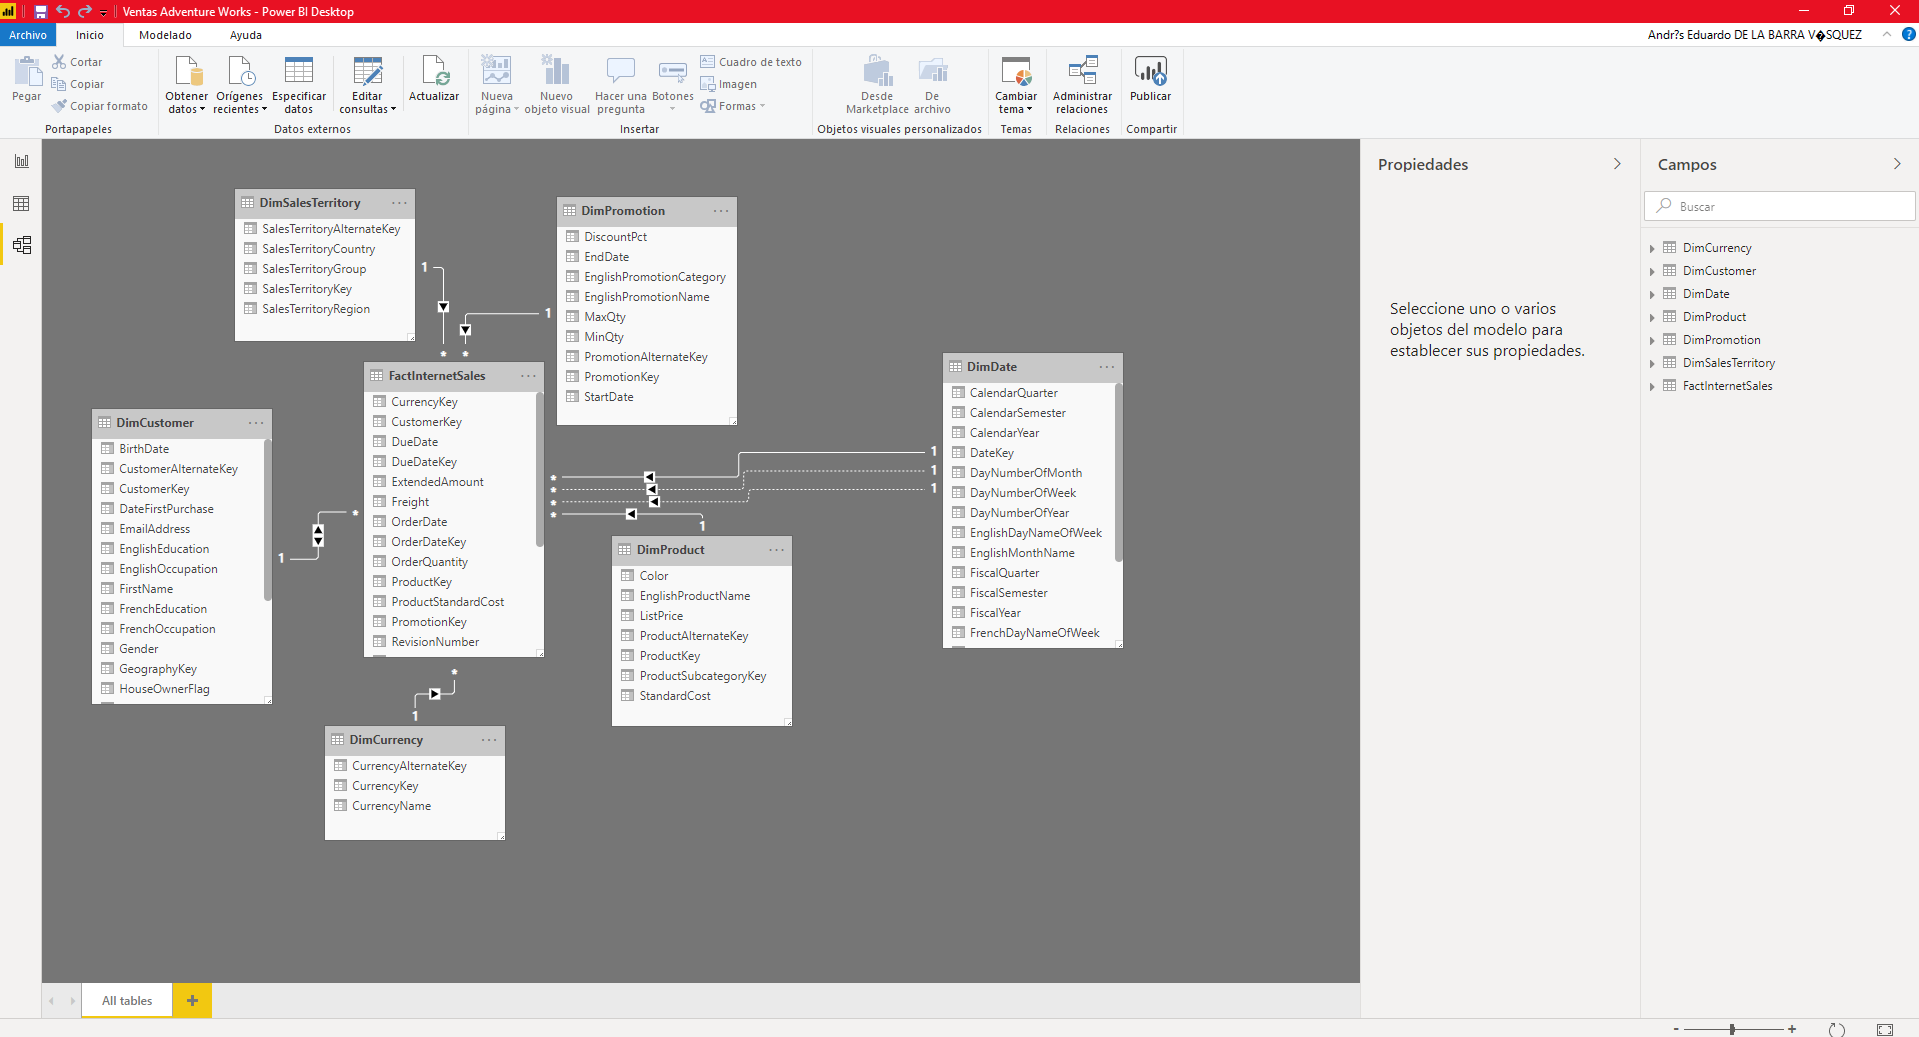
\includegraphics[width=18cm]{./Imagenes/imagen1}
		\end{center}
		\end{figure}

     	\item2. Ejercicio1: Relaciones manuales  
		\begin{figure}[H]
		\begin{center}
		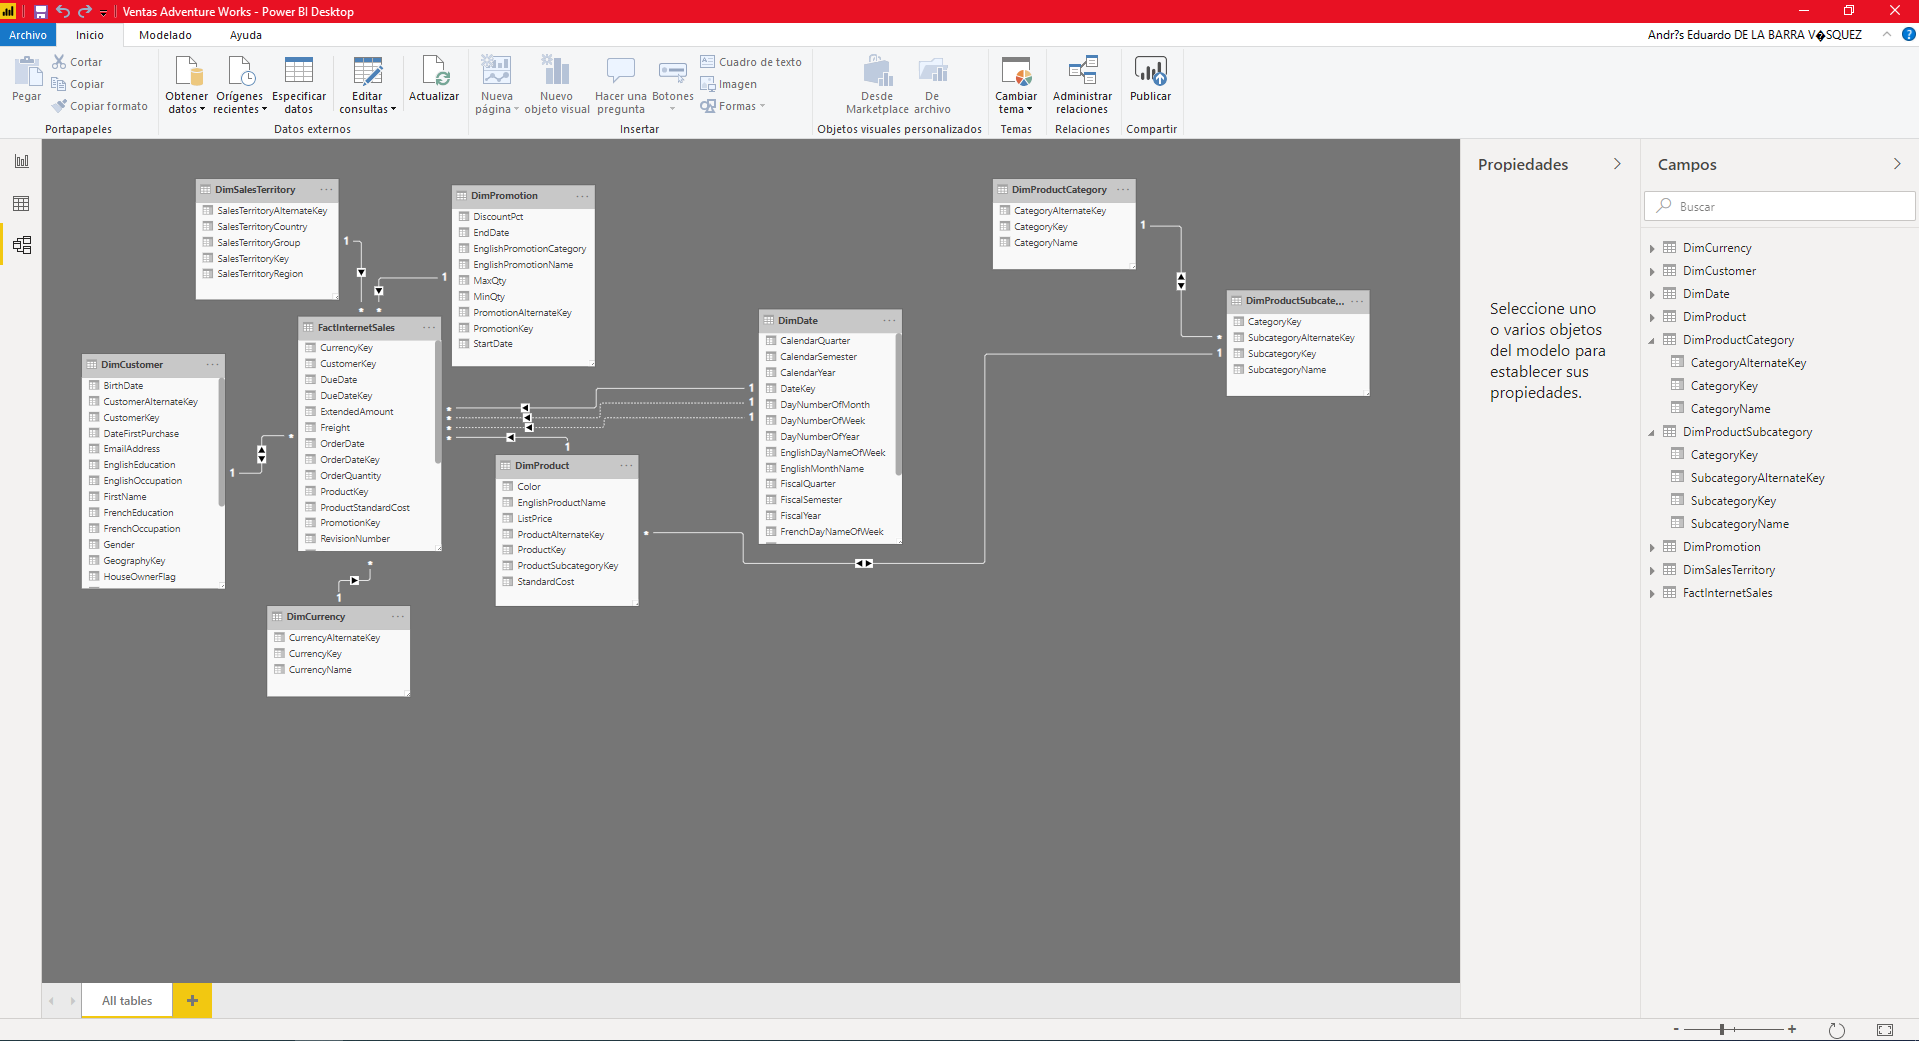
\includegraphics[width=18cm]{./Imagenes/imagen2}
		\end{center}
		\end{figure}
     
	\item3. Ejercicio 2: Query en la tabla DimCustomer
		\begin{figure}[H]
		\begin{center}
		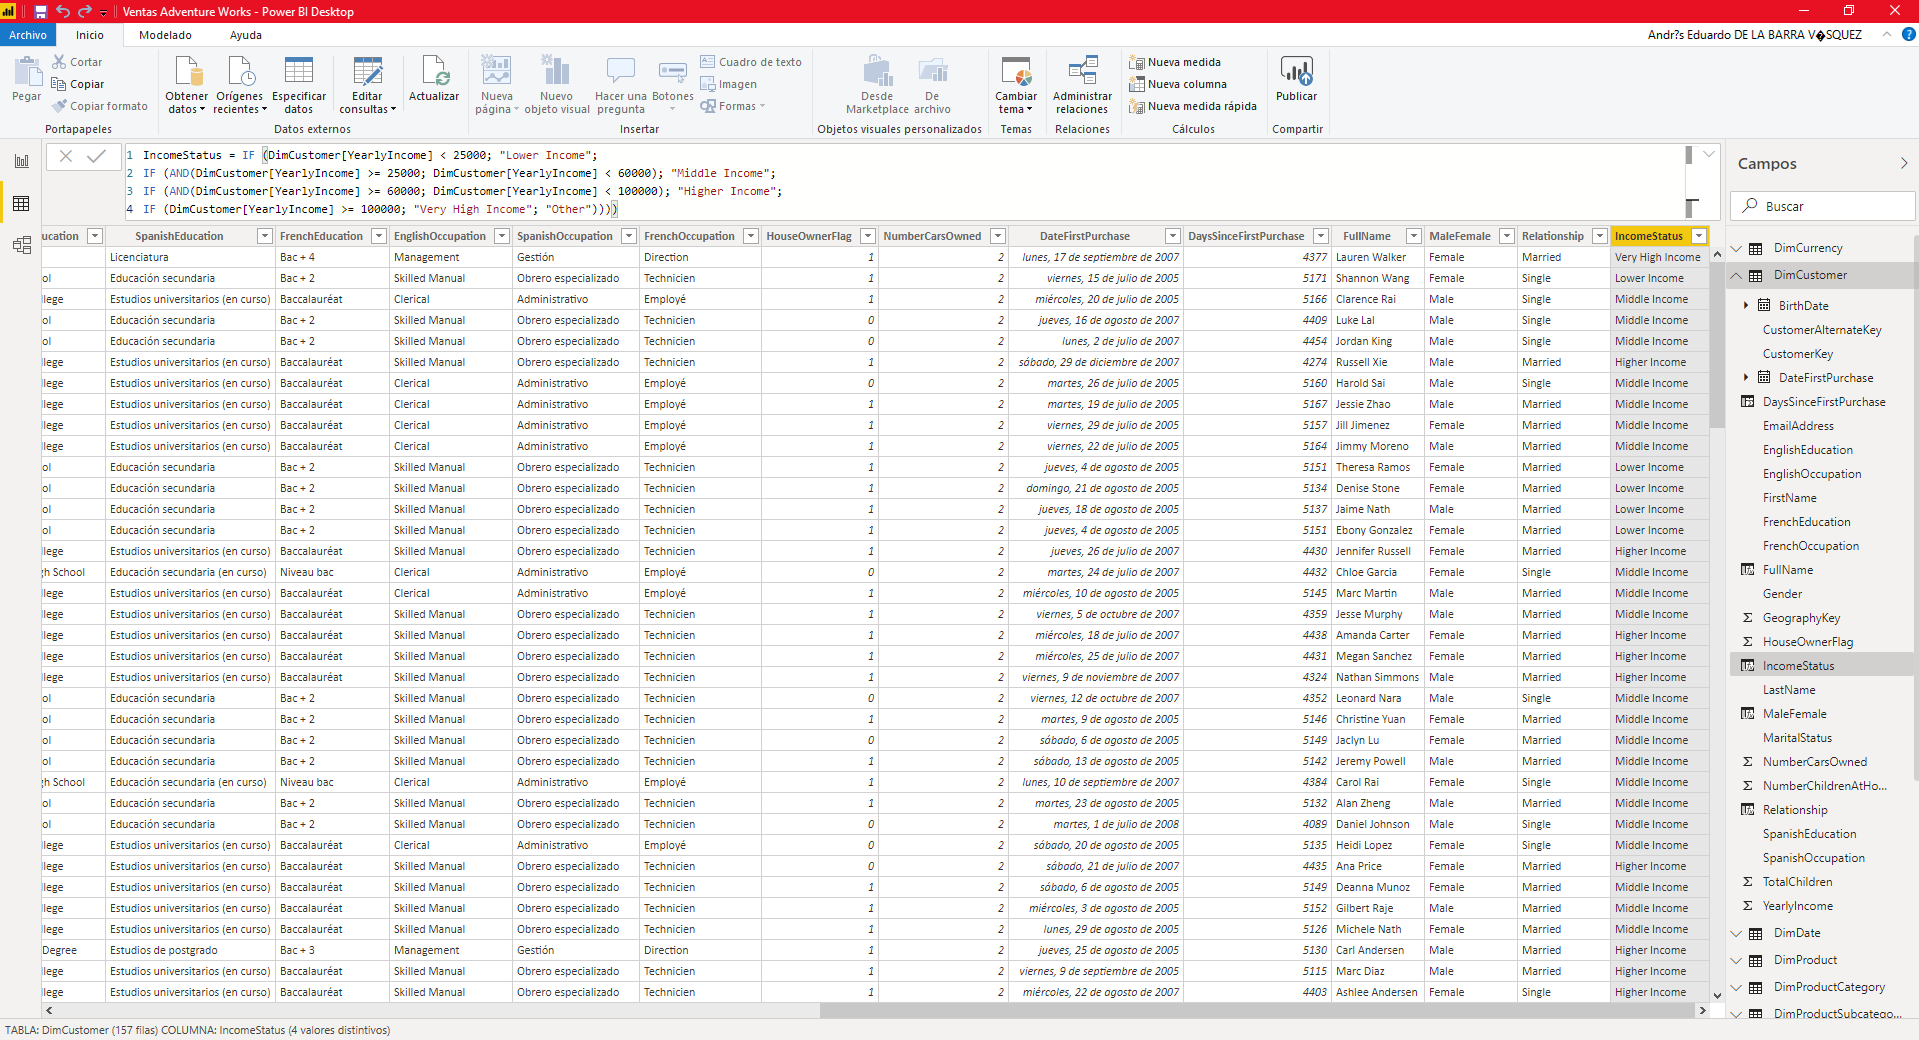
\includegraphics[width=18cm]{./Imagenes/imagen3}
		\end{center}
		\end{figure}
     
	\item 4. Ejercicio 2: Consulta de DimProductSubcategory
		\begin{figure}[H]
		\begin{center}
		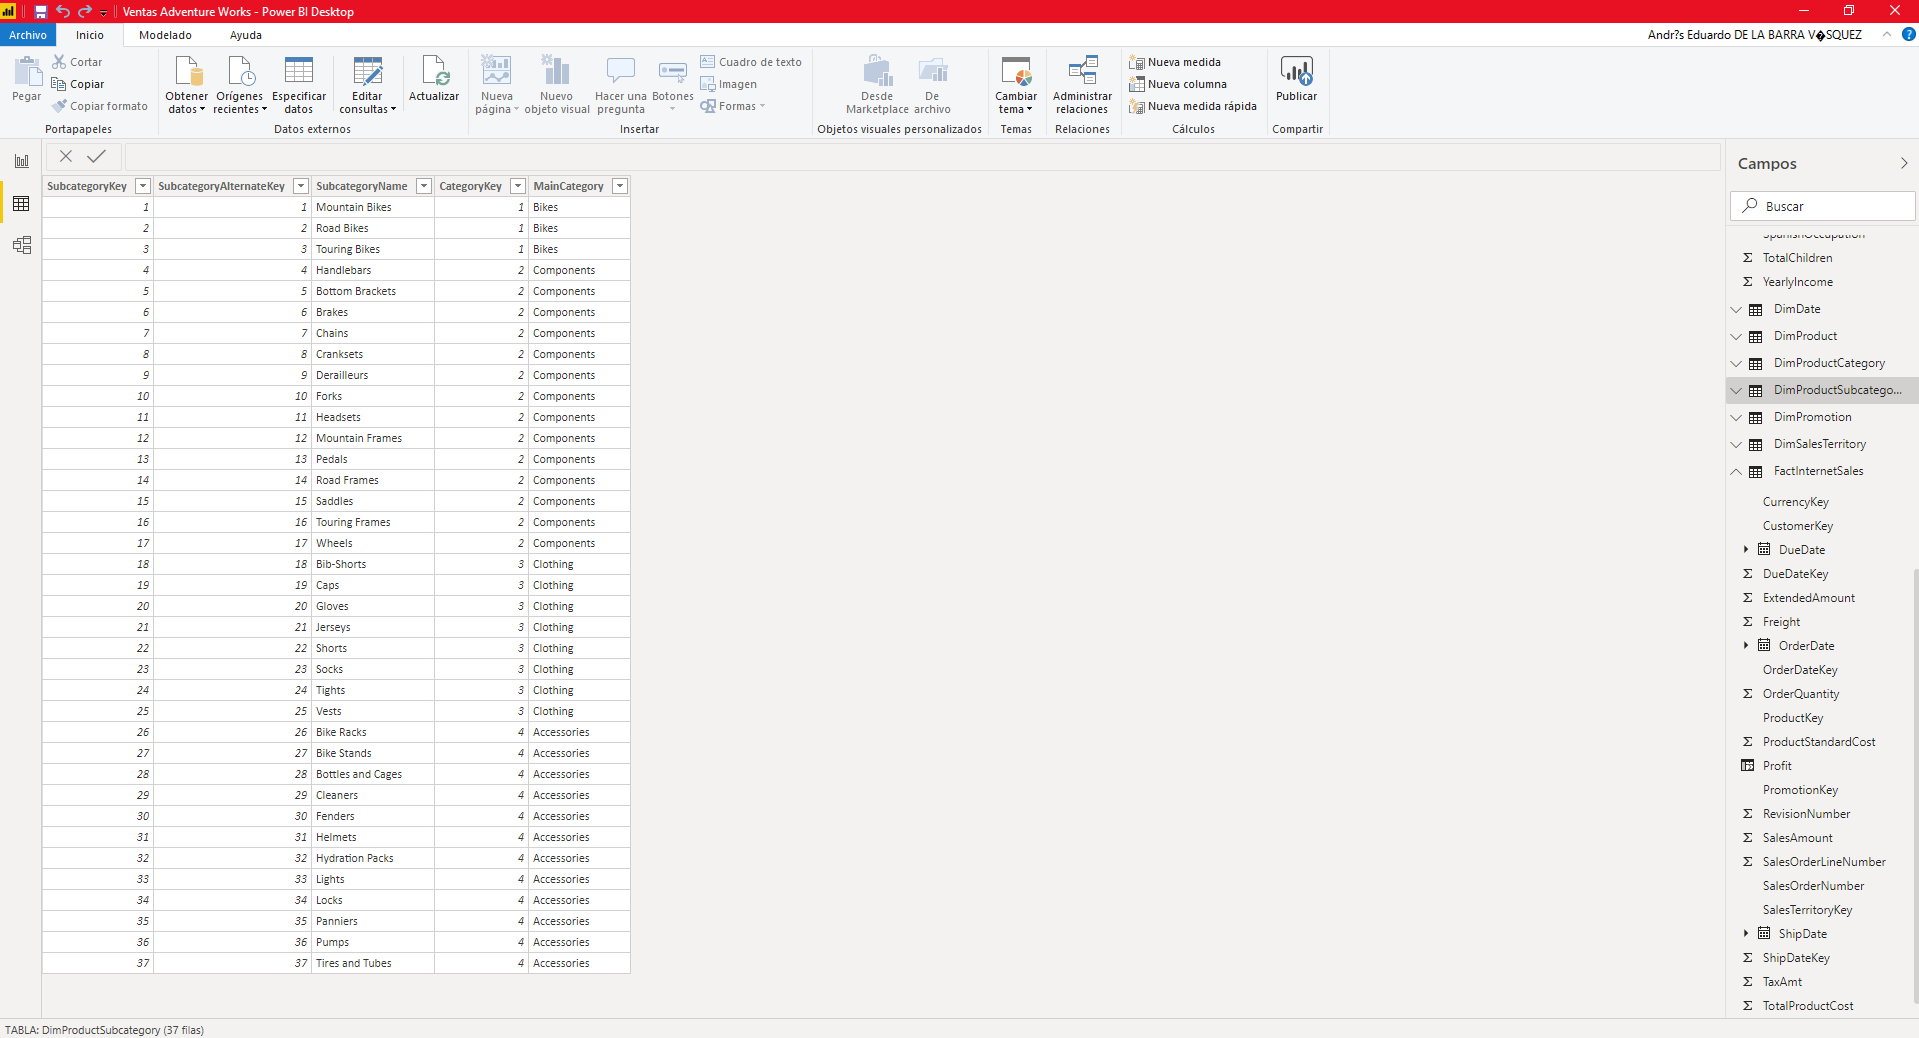
\includegraphics[width=18cm]{./Imagenes/imagen4}
		\end{center}
		\end{figure}
     
	\item 5. Ejercicio 2: Consulta DimPromotion
		\begin{figure}[H]
		\begin{center}
		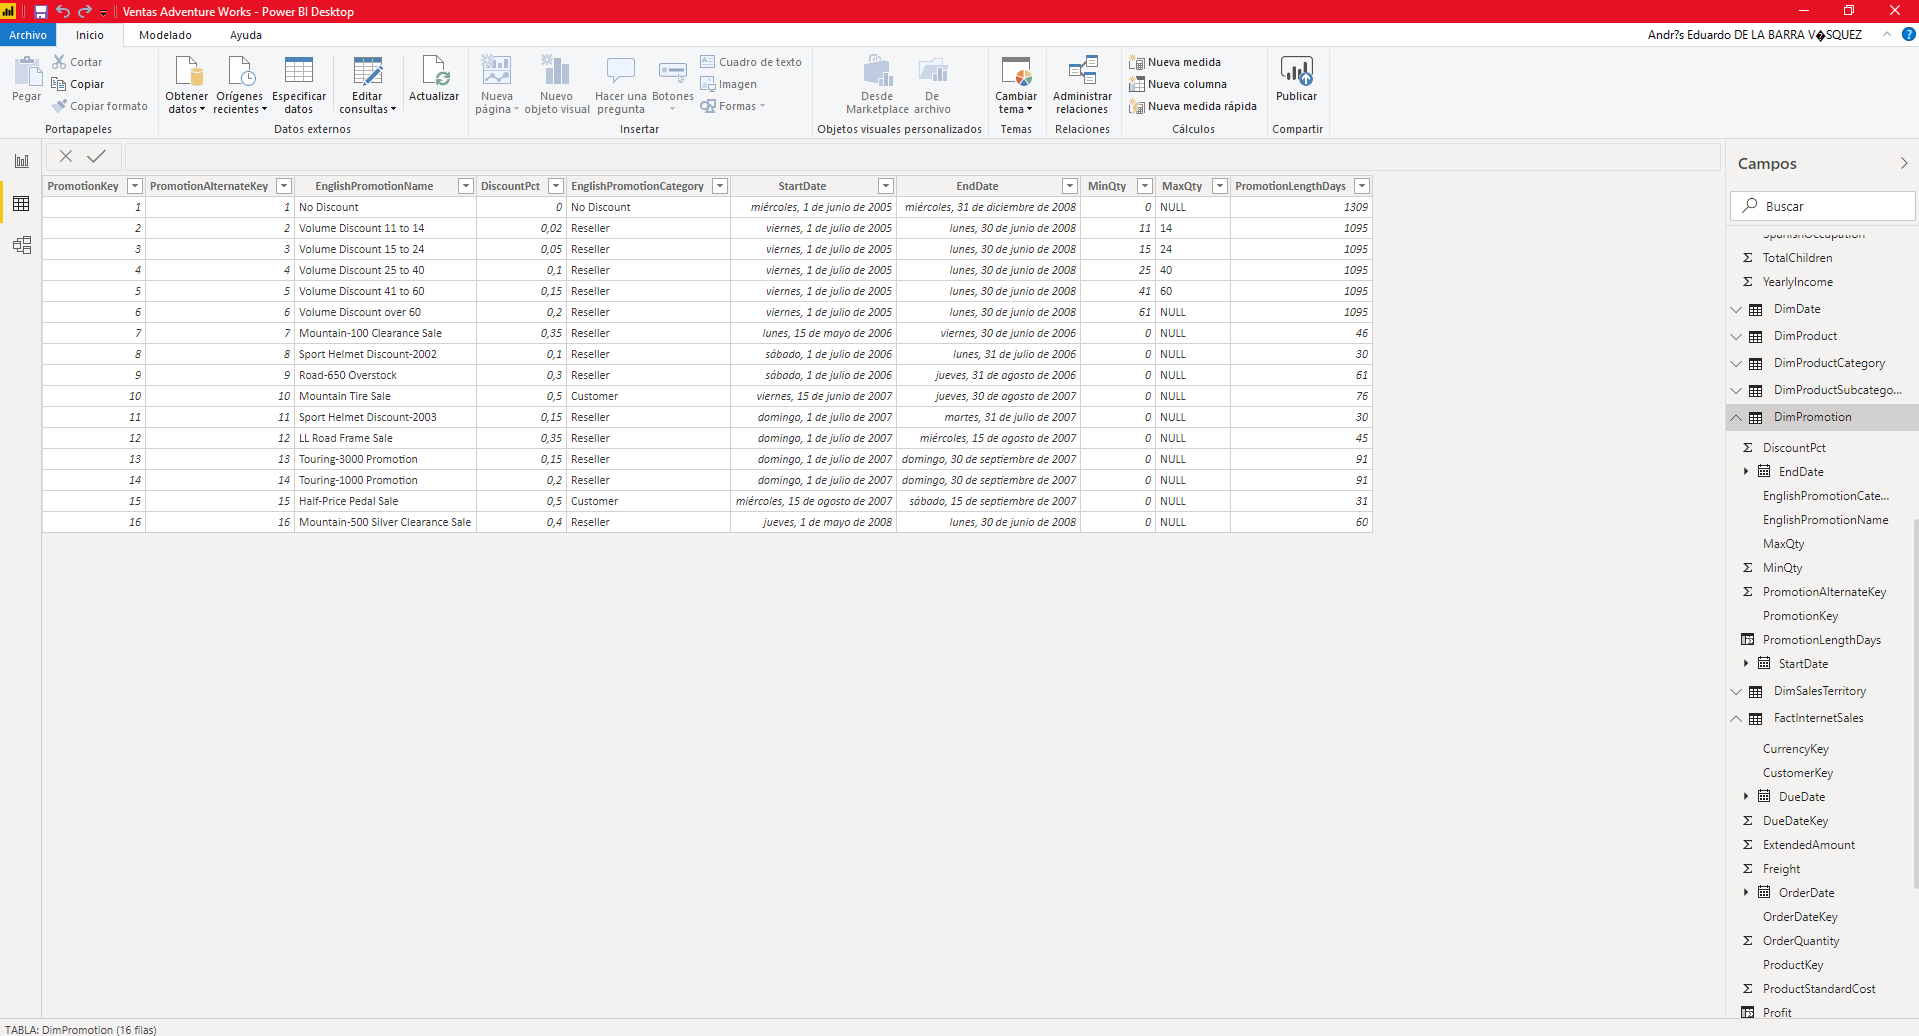
\includegraphics[width=18cm]{./Imagenes/imagen5}
		\end{center}
		\end{figure}
     
	\item 6. Ejercicio 2:Consulta FactInternetSales
		\begin{figure}[H]
		\begin{center}
		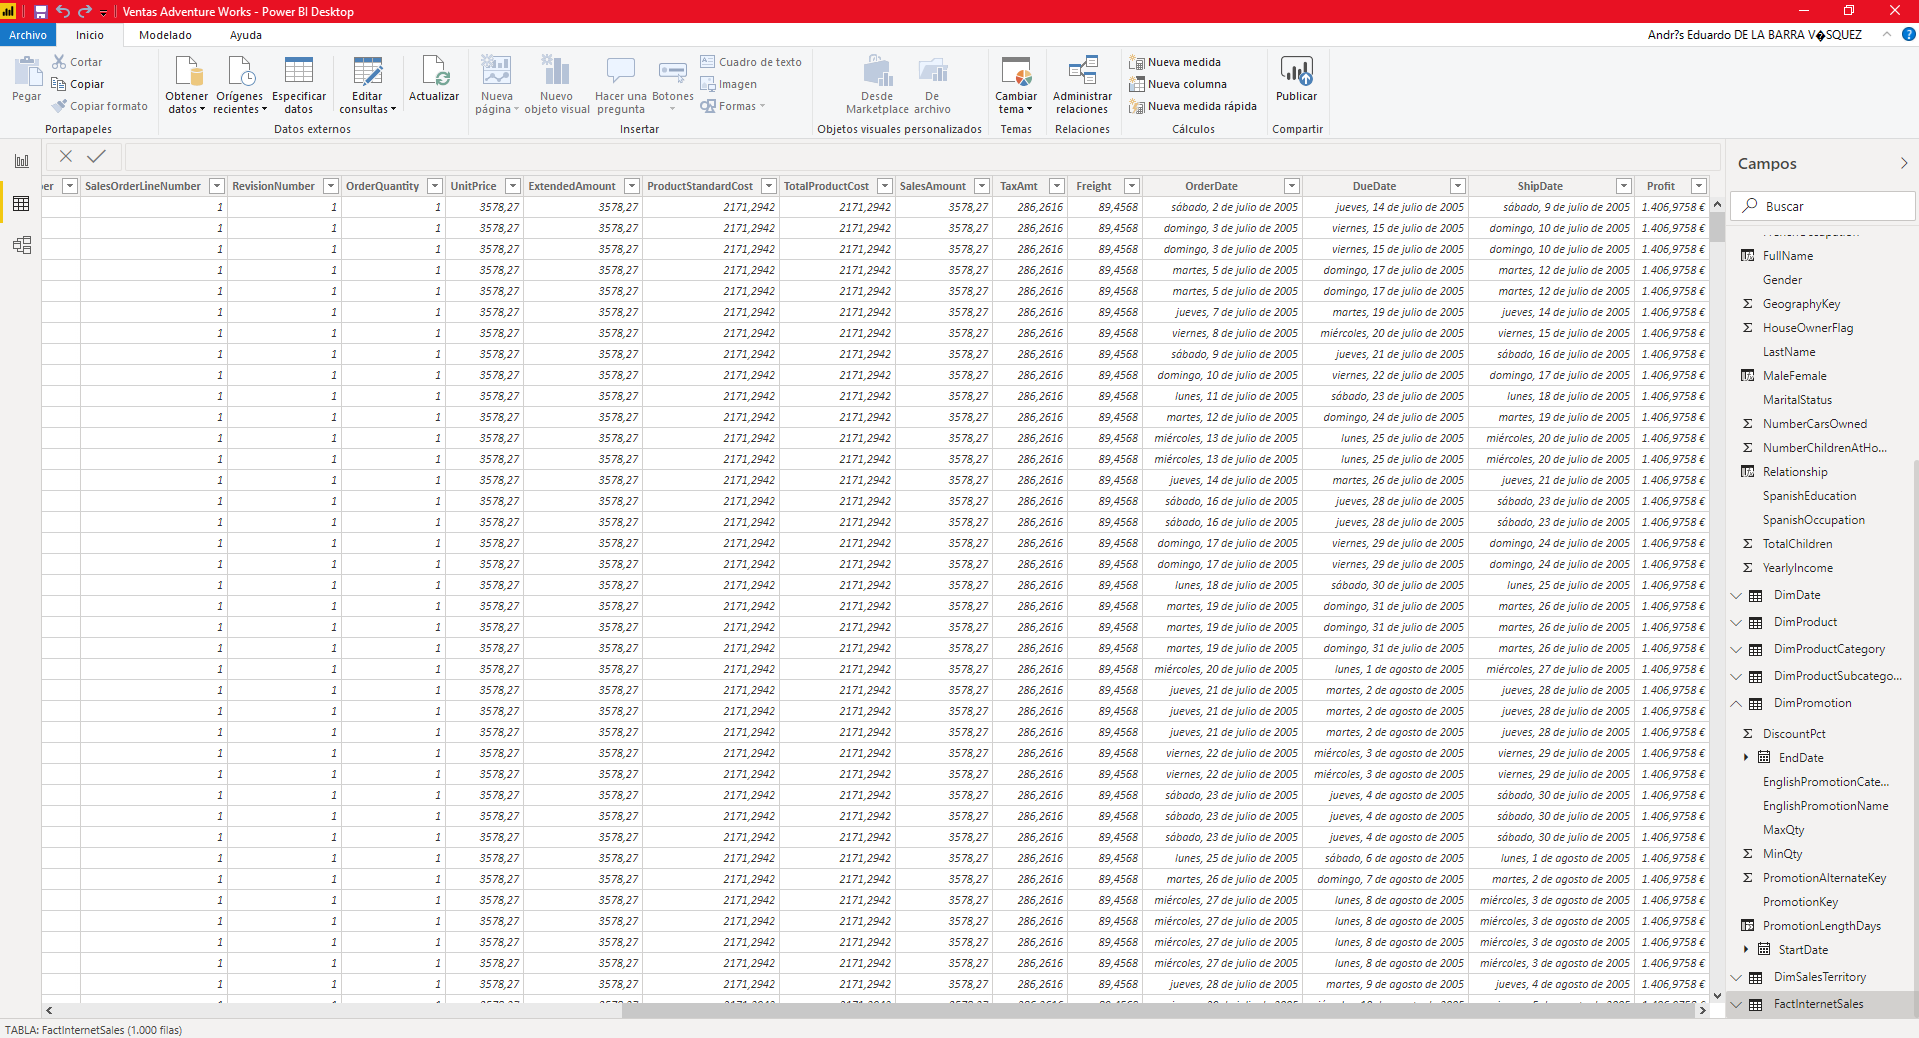
\includegraphics[width=18cm]{./Imagenes/imagen6}
		\end{center}
		\end{figure}
     




\end{itemize}
		